\section{Einleitung}

In diesem Abschnitt werden einige wichtige Begriffe, die im Laufe des
Dokuments auftauchen werden, erl"autert und beschrieben.

\subsection{Grundlagen von WMNs}

\subsubsection{Motivation}

Ein drahtloses vermaschtes Netz (engl. Wireless Mesh Network, WMN) besteht
aus einer Menge von Knoten, die "uber drahtlose Kommunikationstechniken
wie beispielsweise IEEE 802.11 (\ref{ieee80211abg}) Nachrichten
austauschen. Die Vemaschung der Knoten erm"oglicht dabei nicht nur den
Austausch von Nachrichten zwischen unmittelbar benachbarten Knoten,
sondern auch die Vermittlung von Nachrichten an entfernte Knoten "uber
mehrere Knoten hinweg. Die Vermittlungsfunktionalit"at wird dabei oft
von dedizierten Vermittlungsknoten (engl. Mesh-Routern) bereitgestellt,
die somit eine drahtlose Kommunikationsinfrastruktur f"ur die Klienten
(engl. Mesh-Client) bilden. Durch den Einsatz vergleichsweise
kosteng"unstiger Hardwarekomponenten und die Vermaschung der Knoten
erm"oglichen WMNs die kosteng"unstige Vernetzung auch gr"o"serer
Gebiete. Entsprechende Netze werden beispielsweise von Community-Projekten
wie dem Freifunk-Projekt (\ref{other_mesh_projects}) oder Firmen wie
Google (\ref{other_mesh_projects}) bereits heute in der Praxis f"ur den
Aufbau gr"o"serer Netze eingesetzt, um beispielsweise kosteng"unstige
Internetzug"ange f"ur Stadtteile oder ganze St"adte zu realisieren.

WMNs sind auch f"ur den Sonderforschungsbereich (SFB) Nexus an der
Universit"at Stuttgart \cite{nexus} von gro"sem Interesse. Im
Zentrum der Forschungen des SFB stehen Umgebungsmodelle f"ur mobile
kontextbezogene Systeme. Umgebungsmodelle sind digitale Abbilder der
physischen Welt, die von kontextbezogenen Systemen genutzt werden, um
sich selbst"andig an die physische Umgebung des Benutzers anzupassen. Ein
einfaches Beispiel sind ortsbezogene Anwendungen, die beispielsweise
aufgrund der aktuellen geographischen Position eines Ger"ats automatisch
Informationen "uber nahe Restaurants, Sehensw"urdigkeiten, usw. selektieren
k"onnen. Zur Kommunikation, insbesondere mit mobilen Ger"aten, werden dabei
hybride Systeme betrachtet, in denen sowohl eine infrastrukturbasierte
Kommunikation als auch die direkte Ad-hoc-Kommunikation zwischen
mobilen Endsystemen m"oglich ist. Hierbei spielen WMNs als eine spezielle
Auspr"agung eines hybriden Kommunikationssystems eine wesentliche Rolle.

\subsubsection{Drahtloses Ad-Hoc Netzwerk}

Ein drahtloses Ad-Hoc Netzwerk ist ein dezentralisiertes drahtloses Netzwerk.
Das Netzwerk hei"st Ad-Hoc, weil jeder Knoten im Netzwerk Daten
von anderen Knoten im Netzwerk weiterleiten kann, und so wird die Entscheidung,
welcher Knoten die Weiterleitung von Daten eines Knotens "ubernimmt,
dynamisch auf der Grundlage der Netzwerkkonnektivit"at getroffen.
Das Weiterleiten von Paketen in einem Netzwerk "uber mehrere Knoten
nennt man Routing. Und im Gegensatz zu Ad-Hoc Netzwerken "ubernehmen
diese Aufgabe in einem verdrahteten Netzwerk, wie z.B. dem Internet, nur
spezielle Knoten, so genannte Router. Auch in drahtlosen Netzwerken mit
Infrastruktur "ubernehmen diese Aufgabe spezielle Knoten, so genannte
Access Points, die die Kommunikation zwischen drahtlosen Knoten verwalten,
da in solchen drahtlosen Netzwerken Knoten nicht direkt kommunizieren
\cite{toh2001}.

Der dezentralisierte Charakter der drahtlosen Ad-Hoc Netwerken macht sie
f"ur verschiedene Anwendungen geeignet, wo man sich auf zentralisierte Knoten
nicht verlassen kann. Ausserdem verbessert diese Eigenschaft
die Skalierbarkeit der drahtlosen Ad-Hoc Netzen im Vergleich zu
drahtlosen Netzwerken mit Infrastruktur \cite{toh2001}.

Minimale Konfiguration und schnelle Verteilung machen drahtlose Ad-Hoc
Netzwerke geeignet f"ur Notfallsituationen, wie z.B. Naturkatastrophen oder
milit"arische Konflikte. Der Einsatz eines dynamischen und adaptiven
Routing-Protokolls macht es m"oglich, diese Art von Netzwerken schnell
zu installieren \cite{toh2001}.

Drahtlose Ad-Hoc Netzwerke k"onnen in 3 Gruppen unterteilt werden:

\begin{itemize}
\item Mobile Ad-Hoc Networks (MANETs)
\item Wireless Mesh Networks (WMNs)
\item Wireless Sensor Networks (WSNs)
\end{itemize}

Unsere Fachstudie konzentriert sich nur auf WMNs. Deswegen werden diese
Netzwerke im folgenden detaillierter erl"autert.

\subsubsection{WMN}
\label{sec:WMN}

Ein drahtloses vermaschtes Netzwerk ist ein drahtloses Ad-Hoc Netzwerk,
in dem zumindest zwei unterschiedliche Kommunikationspfade zu jedem
Knoten in diesem Netzwerk existieren. Dieser Typ von drahtlosen Ad-Hoc
Netzwerken is sehr zuverl"assig und hat einen sehr hohen Grad an Redundanz.

WMNs bestehen aus Mesh-Routern und Mesh-Clients (Abb. \ref{fig:WMN1}). 
Mesh-Router haben zus"atzliche
Routing-Funktionalit"at, um das Mesh-Netz zu realisieren.
Um die Flexibilit"at des WMNs zu erh"ohen, werden Mesh-Router meistens
mit mehreren drahtlosen Kommunikationsger"aten ausgestattet. Man unterscheidet
zwei Arten von Mesh-Clients: Typ 1 und Typ 2. Mesh-Clients von Typ 1
sind mit einer "aquivalenten Funktionalit"at ausgestattet wie auch
Mesh-Router. Mesh-Clients von Typ 2 sind Knoten mit einer einfacheren
Funktionalit"at als Mesh-Router \cite{toh2001}.

\begin{figure}[H]
\centering
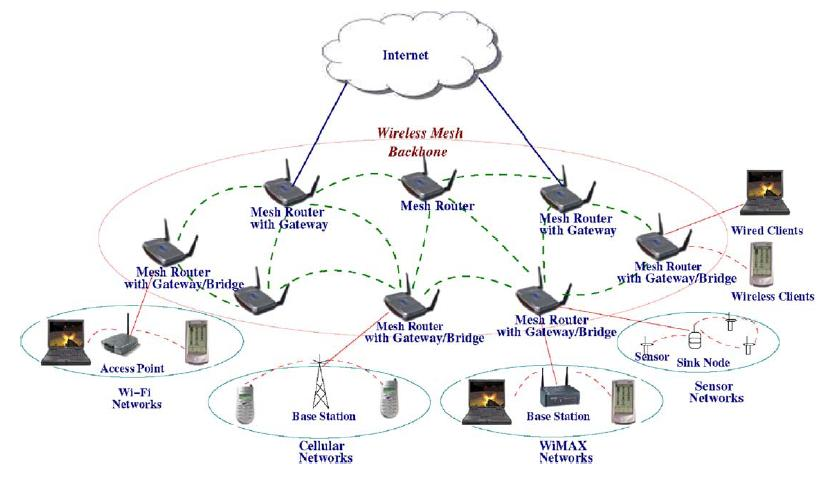
\includegraphics[width=1.0\textwidth]{images/mesh-netz.jpg}
\caption{Mesh-Routern und Mesh-Clients in einem WMN}
\label{fig:WMN1}
\end{figure}

Abh"angig von unterschiedlicher Funktionalit"at von Mesh-Routern und
Mesh-Clients, kann man folgende Architekturen von WMNs unterscheiden
\cite{toh2001}:

\begin{itemize}
\item flache
\item hierarchische
\item hybride
\end{itemize}

Flache WMNs unterst"utzen nur Mesh-Clients von Typ 1, so dass die Funktionen
des WMN wie Routing-, Verwaltung- und Sicherheit-Protokolle f"ur beide
Mesh-Router und Mesh-Clients gleich sind.

Hierarchische WMNs unterst"utzen nur Mesh-Clients von Typ 2. Deswegen sind
die Funktionen von Mesh-Routern und Mesh-Clients sehr unterschiedlich.
Da Mesh-Clients von Typ 2 einige notwendige Funktionen von Mesh-Routern
fehlen, m"ussen Mesh-Router um bestimmte Funktionalit"at erweitert werden,
damit Mesh-Router die Mesh-Clients von Typ 2 unterst"utzen k"onnen.

Hybride WMNs sind verallgemeinerte WMNs und unterst"utzen Mesh-Clients sowohl
von Typ 1 als auch von Typ 2. Auch hier m"ussen Mesh-Router um bestimmte
Funktionen erweitert werden, damit sie die Mesh-Clients von Typ 2
unterst"utzen k"onnen und ihnen einen Zugriffsmechanismus auf das WMN
zur Verf"ugung stellen k"onnen.

Die wichtigsten Eigenschaften von WMNs sind \cite{toh2001}:

\begin{itemize}
\item Multi-Hop drahtloses Netzwerk
\item Hohe Zuverl"assigkeit
\item Hoher Grad an Redundanz
\item F"ahigkeit, sich selbst aufzubauen, zu reparieren und zu
verwalten
\item Kompatibilit"at zu anderen drahtlosen Netzwerken und Integrierbarkeit mit ihnen
\end{itemize}

\subsubsection{IEEE 802.11 Standards}
\label{ieee80211abg}

IEEE 802.11 ist eine Familie von Standards f"ur drahtlose Netzwerke.

Im folgenden werden einige f"ur die Fachstudie wichtige Standards erl"autert.

\paragraph{IEEE 802.11a}\mbox{}

IEEE 802.11a spezifiziert eine Variante der physikalischen Schicht,
die im 5 GHz Frequenzband arbeitet und "Ubertragungsraten bis zu 54 MBit/s
erm"oglicht.

Durch die Verwendung des 5 GHz Ferquenzbereiches kann es zu
St"oreinfl"ussen durch andere Ger"ate, die diese Frequenz benutzen kommen,
z.B. Radarger"ate und Satelliten"ubertragungsger"ate. Deswegen wird der 5
GHz Ferquenzbereich in Europa st"arker als der 2.4 GHz Ferquenzbereich
reguliert.

Es werden 8 nicht "uberlappende Kan"ale im 5 GHz Ferquenzbereich zur
Verf"ugung gestellt. Nicht "uberlappende Funkkan"ale in einem 802.11a WLAN
lassen ca. 3 mal so viele Access Points auf engen Raum zu wie der 802.11b
Standard.

Die zugelassen Sendeleistung durch die ETSI f"ur den 802.11a Standard in
Europa betr�gt 30mW. Dieser Frequenzbereich ist von der RegTP f"ur Lokale
Funknetze am 13. November 2002 geb"uhrenfrei freigegeben worden.
In Deutschland ist die Nutzung dieser Norm nur auf den Einsatz im
Indoorbereich beschr"ankt.

\paragraph{IEEE 802.11b}\mbox{}

IEEE 802.11b ist ebenfalls eine alternative Spezifikation der physikalischen
Schicht, die mit dem bisher genutzten 2.4 GHz Frequenzband auskommt und
"Ubertragungsraten bis zu 11 MBit/s erm"oglicht. 

Eine Kompatibilit"at zwischen dem 802.11a und 802.11b besteht wegen
unterschiedlicher "Ubertragungsfrequenzen nicht.

Es werden nur 3 nicht "uberlappende Kan"ale zur Verf"ugung gestellt,
wodurch es bei einer gr"o"seren Fl"achendeckung mit 802.11b
Access Points zu Interferenzen mit anderen Access Points, die auf den selben Kan"alen
senden, kommt.

Das 2.4 GHz Frequenzband teilen sich unter anderem z.B.
Mikrowellenherde und Bluetooth-Ger"ate, welchee ebenfalls eventuelle
St"orungen hervorrufen k"onnten. Ger"ate mit dieser Norm d"urfen in Deutschland
f"ur den Indoor- sowie Outdoorbereich genutzt werden. 

\paragraph{IEEE 802.11g}\mbox{}

IEEE 802.11g spezifiziert eine Variante der physikalischen Schicht,
die im 2.4 GHz Frequenzband arbeitet und "Ubertragungsraten bis zu 54 MBit/s
erm"oglicht.

Zwischen dem 802.11b und 802.11g Standard besteht v"ollige
Abw"artskompatibilit"at durch Verwendung der CCK-Modulation.

Die Nutzung von Ger"aten mit dieser Norm ist f"ur den Indoor- und
Outdoorbereich von der RegTP genehmigt worden.

\paragraph{IEEE 802.11n}\mbox{}

IEEE 802.11g spezifiziert eine Variante der physikalischen Schicht,
die vorzugsweise im 5 GHz Frequenzband arbeitet, MIMO-Technologie einsetzt
und "Ubertragungsraten bis zu 500 MBit/s erm"oglicht.

MIMO sendet mit mehreren Antennen in verschiedene Richtungen und Wege.
Der MIMO Empf"anger besitzt ebenfalls mehrere Antennen, um die Signale
wieder zu empfangen und durch eine digitale Signalaufbereitung wieder zu
entschl"usseln. Bei MIMO steigt der Datendurchsatz linear zur verwendeten
Antennenanzahl an.

IEEE 802.11n befindet sich noch in Entwicklung.

\paragraph{IEEE 802.11s}\mbox{}

IEEE 802.11s ist ein Standard f"ur drahtlose vermaschte Netzwerke.
Der Standard spezifiziert WMNs auf der Sicherungsschicht (Layer 2).

IEEE 802.11s Standard basiert auf IEEE 802.11a/b/g Standards und ist 
kompatibel mit diesen Standards.

\subsubsection{Ad-Hoc Routing-Protokolle}

Ein Ad-Hoc Netzwerk, beispielsweise ein Sensornetzwerk, besteht aus einer
gro"sen Anzahl von Knoten, die sich typischerweise spontan vernetzen
m"ussen. "Uber Funk k"onnen diese Knoten miteinander kommunizieren. 
Knoten k"onnen aber wegen der Leistungsf"ahigkeit, des Energieverbrauches
und auch der Mobilit"at nicht mit allen anderen Knoten direkt kommunizieren.
Routing-Verfahren bieten die M"oglichkeit, Kommunikation
zwischen zwei Knoten mit Hilfe der anderen Knoten auszuf"uhren, wenn
beide Knoten miteinander nicht direkt kommunizieren k"onnen.
Mit anderen Worten erlaubt Routing indirekte Kommunikation zwischen
Knoten in einem Netzwerk \cite{toh2001}.

Es gibt mehr als 70 konkurrierende Entw"urfe f�r das Routing der Pakete
durch ein Mobiles Ad-Hoc/Maschennetzwerk. Eine Klassifikation der
Routingprotokolle kann durch die Anzahl der Empf"anger getroffen werden:
\begin{itemize}
\item unicast Routing - Ziel der Daten"ubertragung ist ein einzelner Knoten
\item multicast Routing - Ziel sind mehrere Knoten
\item geocast Routing - Ziel sind alle Knoten in einem bestimmten
geografischen Bereich
\item broadcast Forwarding - Ziel sind alle Knoten in der Reichweite
des Senders
\end{itemize}

Eine andere M"oglichkeit der Klassifikation besteht in der Einteilung
der Protokolle hinsichtlich des grunds"atzlichen Ansatzes. Diese Ans"atze
werden im Folgenden vorgestellt.

\paragraph{Positionsbasierte Routingverfahren}\mbox{}

Positionsbasierte Routingverfahren nutzen geod"atische Informationen "uber
die genauen Positionen der Knoten. Diese Informationen werden z.B. "uber
GPS-Empf"anger gewonnen. Anhand dieser Ortsinformationen l"asst sich der
k"urzeste oder der beste Pfad zwischen Quell- und Zielknoten bestimmen. Ein
Beispiel f"ur ein positionsbasiertes Routingprotokoll ist Location Aide Routing
(LAR) \cite{toh2001}.

\paragraph{Topologiebasierte Routingverfahren}\mbox{}

Die topologiebasierten Routingverfahren kommen ohne geod"atische
Informationen "uber die Positionen der Knoten des mobilen
Ad-hoc-Netzes aus. Ihnen gen"ugen logische Informationen "uber die
Nachbarschaftsbeziehungen der Knoten, also welche Knoten eine direkte
Verbindung haben oder "uber einen oder mehrere Zwischenknoten (hops)
in Verbindung treten k"onnen. Diese Nachbarknoten k"onnen miteinander
kommunizieren. Die topologischen Informationen werden meistens durch
den Versand so genannter HELLO-Pakete gewonnen. Je nach Zeitpunkt des
Aufbaus der Topologiedatenbasis handelt es sich um proaktives oder
reaktives Routing. Ein Beispiel f"ur ein Protokoll aus dieser Klasse ist
das Neighbourhood Discovery Protocol (NHDP), das Elemente des Optimized
Link State Routing Protocol (OLSR) verwendet \cite{toh2001}.

\paragraph{Proaktive Verfahren}\mbox{}

Proaktive Routingverfahren bestimmen die zu verwendenden Pfade zwischen
zwei Knoten bereits, bevor diese f"ur die "Ubertragung von Nutzdaten
ben"otigt werden. Sollen dann Nutzdaten verschickt werden, so muss nicht
auf die Bestimmung des Pfads zum Zielknoten gewartet werden. Nachteilig
ist daf"ur jedoch, dass diese Verfahren auch ohne Verkehr von Nutzdaten
viele Kontrollpakete verschicken, um Pfade zu bestimmen, die wom"oglich
sp"ater nicht ben"otigt werden. Ein Beispiel f"ur ein Protokoll aus dieser
Klasse ist OLSR \cite{toh2001}.

\paragraph{Reaktive Verfahren}\mbox{}

Im Gegensatz zu den proaktiven Verfahren bestimmen reaktive
Routingverfahren die ben"otigten Pfade zwischen
zwei Knoten erst, wenn Nutzdaten "ubertragen werden sollen. Daraus ergibt
sich, dass das erste Datenpaket einer Verbindung erst mit Verz"ogerung
versendet werden kann, da zun"achst auf den Abschluss der Routenbestimmung
gewartet werden muss. Daf"ur werden allerdings auch nur Kontrollpakete
versendet, wenn Nutzdaten verschickt werden und dies zur Routenbestimmung
notwendig ist. Dies schl"agt sich positiv im Energieverbrauch der Knoten
nieder. Das Protokoll Ad hoc On-Demand Distance Vector (AODV) ist ein
Beispiel f"ur ein Protokoll dieser Kategorie \cite{toh2001}.

\paragraph{Hybride Verfahren}\mbox{}

Hybride Verfahren kombinieren proaktive und reaktive
Routingverfahren. Dabei soll das Ziel erreicht werden, die
Vorteile der beiden Ans"atze in einem neuen Routingprotokoll
zusammenzufassen. Beispielsweise kann in einem lokal beschr"ankten Bereich
ein proaktives Verfahren eingesetzt werden, w"ahrend f"ur weiter entfernte
Ziele ein reaktives Verfahren eingesetzt wird. Dies vermindert die
Belastung des Netzes durch Kontrollpakete, die bei einem rein proaktiven
Verfahren "uber das gesamte Netz versendet w"urden. Trotzdem stehen f"ur
lokale Ziele sofort Pfade zur Verf"ugung, ohne dass auf deren Bestimmung
wie bei einem rein reaktiven Verfahren gewartet werden m"usste.
Zone Routing Protocol (ZRP) ist ein Routingprotokoll,
das diesen Ansatz umsetzt \cite{toh2001}.

\paragraph{OLSR}\mbox{}

\begin{figure}[H]

\includegraphics{Olsrd_logo.png}
\end{figure}

Optimized Link State Routing, kurz OLSR, ist ein Routingprotokoll
f"ur mobile Ad-hoc-Netze, das eine an die Anforderungen eines mobilen
drahtlosen LANs angepasste Version des Link State Routing darstellt. Es
wurde von der IETF mit dem RFC 3626 standardisiert. Bei diesem
verteilten flexiblen Routingverfahren ist allen Routern die vollst"andige
Netztopologie bekannt, sodass sie von Fall zu Fall den k"urzesten Weg zum
Ziel festlegen k"onnen. Als proaktives Routingprotokoll h"alt es die daf"ur
ben"otigten Informationen jederzeit bereit. Ein in Mesh-Netzen
bekannter Vertreter von LSR ist OLSR von olsr.org. Inzwischen existieren
f"ur OLSR spezielle Erweiterungen. Mit der ETX-Erweiterung wird dem
Umstand Rechnung getragen, dass Links asymmetrisch sein k"onnen. Mit
dem Fisheye-Algorithmus ist OLSR auch f"ur gr"o"sere Netzwerke brauchbar
geworden, da Routen zu weiter entfernten Knoten weniger h"aufig neu
berechnet werden. Der entscheidende Nachteil ist aber der trotz
Fisheye-Algorithmus noch recht hohe Rechenaufwand des OLSR Routing-Daemon,
sobald die Anzahl an Knoten ein gewisses Ma"s ubersteigt.

\paragraph{B.A.T.M.A.N.}\mbox{}

\begin{figure}[H]
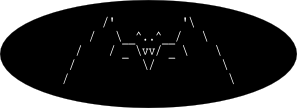
\includegraphics{Batman_logo.png}
\end{figure}

B.A.T.M.A.N., Better Approach To Mobile Adhoc Networking, ist
ein Routing-Protokoll f"ur mobile Ad-Hoc Netzwerke. B.A.T.M.A.N.
wird von der Gemeinde des FreiFunk-Projektes entwickelt. Dieses
neue Routing-Protokoll soll das OLSR-Protokoll abl"osen, das zur Zeit
im FreiFunk-Netzwerk verwendet wird. Das FreiFunk-Netzwerk ist
inzwischen so gro"s geworden, dass das FreiFunk-Projekt
auf Skalierbarkeitsprobleme wegen der Schw"achen von OLSR-Protokoll
gestossen ist. B.A.T.M.A.N. berechnet im Gegensatz zu OLSR
Routing-Protokoll keine Routen im voraus und es werden keine Routing-Information
wie bei OLSR im ganzen Netzwerk geflutet. Jeder Knoten im Netzwerk
kennt nur seine direkten Nachbar. B.A.T.M.A.N. soll das Skalierbarkeitsproblem
von OLSR l"osen und OLSR-Protokoll im FreiFunk-Netzwerk abl"osen
\cite{elektra2007,batman}.

\subsection{Existierende L"osungen und Projekte}
\label{other_mesh_projects}

\begin{description}

\item[FreiFunk]
hat zum Ziel, freie, unabh"angige und nichtkommerzielle Computer-Funknetze
zu etablieren.  Es bildet eine Plattform f"ur Menschen, die an einer
offenen Netzwerk-Infrastruktur interessiert sind.

\url{http://wiki.freifunk.net/Hauptseite}

\item[OpenNet]
hat sich zur Aufgabe gemacht, freie und offene
Kommunikationsinfrastrukturen zu f"ordern. Dabei setzen die
Vereinsmitglieder auf WLAN-Technik und die Vernetzung von Dach zu Dach
und Haus zu Haus.

\url{http://wiki.opennet-initiative.de/index.php/Hauptseite}

\item[UMIC-Mesh]

ist ein hybrides Testbed f"ur WMNs.
Das Projekt verfolgt 2 Ziele, einerseits ein gro"ses und sklalierbares
Ad-Hoc Mesh-Netz f"ur Forschung bereitzustellen und andererseits
allen Studenten und Mitarbeiter der Computer Science Abteilung
an der RWTH Aachen Universit"at einen breitbandigen Zugang zum Netzwerk
der Abteilung zur Verf"ugung zu stellen.


\url{http://umic-mesh.net/}

\item[Google WiFi]

ist ein freies WMN, das von Google finanziert wird und zur Zeit in
Mountain View in Kalifornien eingesetzt wird.

\url{http://wifi.google.com/}

\end{description}
